\chapter{Implementatie}
In het vorige hoofdstuk is er beschreven hoe de architectuur van een monitoring library eruit kan zien. In dit hoofdstuk wordt er gekeken naar de implementatie van de Tracklytics library. %\cite{tracklytics}
Er wordt gekeken naar welke technologie\"en er gebruikt zijn bij het ontwikkelen van de library. Daarnaast wordt er uitgelegd hoe developers de library kunnen gebruiken in hun applicaties. Er wordt dieper ingegaan op de communicatie tussen de Tracklytics library en de server.

\section{Details Implementatie}
In deze sectie wordt er besproken welke technologie\"en er gebruikt zijn bij het ontwikkelen van de Tracklytics library.

\subsection{iOS Library}
De Tracklytics library beschreven in deze thesis is ontwikkeld voor het iOS besturingssysteem. Voor het iOS besturingssysteem bestaan er twee programmeertalen om een applicatie, of in dit geval een library, te ontwikkelen, namelijk: Swift en Objective-C. Swift is een redelijk recente taal, op het moment van schrijven is deze nog geen twee jaar oud. Omdat de ondersteuning van Swift door de meerderheid van de developers nog zeer karig is, is er besloten om de library in Objective-C te schrijven. Objective-C en Swift hebben dezelfde functionaliteiten, maar programmeren in Swift is overzichtelijker door de andere syntax. Swift is meer ge\"integreerd in de IDE die Apple aanbiedt om applicaties mee te ontwikkelen. Swift is veiliger en sneller dan Objective-C. Al deze redenen pleiten om Swift als programmeertaal te kiezen. Het grote nadeel is dat Swift nog niet in veel applicaties aanwezig is en dat het moeilijker is om in een Swift applicatie een Objective-C library te integreren dan andersom. Dit is de grote reden waarom er voor Objective-C gekozen is.\\
%cite swift

De Tracklytics library slaat tijdelijk de data op op de harde schijf van het toestel. Dit heeft twee voordelen, namelijk: er gaat geen data verloren en de library gebruikt minder RAM.
Als het toestel geen internet connectie zou hebben, kan de library de data niet verzenden naar de back end en indien de applicatie dan sluit zijn alle gegevens verloren. Dit scenario is opgelost door het tijdelijk opslaan van de gegevens op de harde schijf. De data wordt pas verwijderd als de library er zeker van is dat de data succesvol naar de back end is verstuurd. 

Een mobiel toestel heeft een beperkte grootte RAM geheugen en applicaties kunnen hier niet volledig gebruik van maken omdat het besturingssysteem dit geheugen ook gebruikt. Als de applicatie teveel RAM geheugen gebruikt, dan gaat heel de applicatie deze trager werken, omdat het RAM geheugen dan uitgeswapt wordt naar de harde schijf. Het is dus noodzakelijk om het RAM gebruik zo laag mogelijk te houden. Indien alle data in RAM geheugen zou gehouden gestoken worden, dan kan dit snel vollopen. Het opslaan van de data op de harde schijf verhelpt dit probleem. Het is dan wel noodzakelijk dat het opslaan van de data op schijf in de achtergrond gebeurt, omdat I/O operaties relatief lang duren. \\

De methodes van de Tracklytics library die gebruikt kunnen worden zijn statische methodes. De keuze hiervoor is gebaseerd op twee redenen.

De Tracklytics library klasse die de methodes aanbiedt is geen objectgerichte klasse. Indien er een object van deze klasse zou gemaakt worden, zou deze elke keer na creatie bijna onmiddelijk niet meer gebruikt worden. Deze creatie van het object zorgt voor een overhead, de welke is weggewerkt door het statisch maken van alle methodes die bruikbaar zijn door de developers. 

Een tweede reden is de gebruiksvriendelijkheid. Een library call neemt maar \'e\'en lijn code in om een methode uit te voeren in plaats van twee. Dit zorgt voor minder code. De impact hiervan hangt af van het aantal monitoring punten die in de applicatie zijn ingevoerd. Dit verbetert ook de leesbaarheid van de code.\\

\subsection{Back end}
De data die de Tracklytics library doorstuurt vanaf het toestel van de gebruiker moet opgeslagen worden in een database. Zo kan deze data later verwerkt worden en worden weergegeven in het dashboard. Er moet een keuze gemaakt worden over het besturingssysteem, de database en de programmeertaal van de back end.\\

De server draait in OpenStack, een cloud platform. Deze is gedeployed als infrastructure-as-a-service (IaaS). Dit wil zeggen dat dit meerdere virtuele servers kan aanbieden (zelfs meerdere virtuele servers als fysieke servers). Dit biedt een abstractie en schermt de virtuele server af van andere virtuele servers. Een gebruiker kan zelf nieuwe virtuele servers aanmaken. Elke virtuele server heeft zijn eigen besturingssysteem, te kiezen uit een lijst van images aangeboden door OpenStack. 
%\cite openstack

In de Tracklytics architectuur is gekozen voor een linux distributie (in dit geval Ubuntu). Deze keuze is gemaakt op basis van de gebruiksvriendelijkheid van dit besturingssysteem. Zo is het gemakkelijk om snel een webserver op te zetten en een database te installeren. Er is voor Ubuntu gekozen, omdat dit de meest gekende en meest gebruikte linux distributie is. \\
%\cite ubuntu

In de database wordt alle data opgeslagen, wat wil zeggen dat dit een van de meest belangrijke onderdelen van de Tracklytics architectuur vormt. De metadata die gecollecteerd wordt per applicatie is in vele gevallen hetzelfde. De parameters die verschillen zijn: het type toestel, het type internet connectie en de versie van de applicatie. Dit gegeven zorgt ervoor dat de metadata vaak hetzelfde is. Indien de metadata uit de data komende van de Tracklytics library wordt uitgehaald kan er relatief veel opslagruimte gespaard worden, omdat deze metadata niet in elke entry in de database aanwezig moet zijn, enkel een verwijzing naar waar die metadata staat. Er is gekozen om een MySQL database te gebruiken, omdat deze een gestructureerde tabellenstructuur heeft en zo de metadata gemakkelijk van de data kan scheiden. De data kunnen door SQL queries gecombineerd worden in views om de data overzichtelijk te maken. Een alternatief is een NoSQL database. Dit alternatief past niet in de manier waarop de data opgeslagen wordt, omdat deze een niet-gestructureerde database aanbiedt. \\

De back end heeft in de Tracklytics library twee functies, namelijk: het verwerken en opslaan van de data in de database en het opvragen van data uit de database om het dashboard van de data te voorzien. De keuze is gevallen op PHP als programmeertaal. Met PHP is het simpel om een database connectie op te zetten en via SQL queries deze dat in of uit de database te krijgen. Een tweede voordeel van PHP is dat deze met POST data om kan. Via deze manier kan de data in de request van de Tracklytics library verborgen worden in de request en moet deze niet rechtstreeks doorgegeven worden in bijvoorbeeld de URL zelf. Zo is er meer veiligheid en privacy van de data. \\


\subsection{Dashboard}\label{visualisatie}
Het Tracklytics dashboard is ontworpen om de gegevens van de applicatie in grafieken en details weer te geven om hieruit een conclusie te kunnen trekken over het functioneren van de applicatie. Het dashboard is ontworpen als webapplicatie in plaats van een desktop applicatie. De voordelen hiervan zijn: software updates automatisch worden doorgevoerd zonder dat er tussenkomst van de gebruiker nodig is, het is cross platform, omdat het in de browser draait en er is geen installatie vereist. \\

Om de webapplicatie te ontwikkelen is er gebruik gemaakt van AngularJS. De reden hiervoor is dat dit een zeer handig framework is voor het ontwikkelen van dynamische websites. Dit framework bindt stukken HTML code aan JavaScript code, wat ervoor zorgt dat het DOM gemakkelijk manipuleerbaar is door JavaScript. Een tweede reden waarom AngularJS in deze situatie voordelig is, is dat met AngularJS het gemakkelijk is om stukken HTML te laten herhalen met andere gegevens in. Zo kunnen de verschillende grafieken onder elkaar geplaatst worden zonder telkens de HTML code in JavaScript aan te moeten passen. Een bijkomstig voordeel is dat de data in de verschillende tabbladen maar eenmalig ingeladen moet worden, omdat AngularJS ervoor zorgt dat als je op een tab drukt niet de hele webpagina opnieuw wordt ingeladen, maar enkel de view die verandert ingeladen wordt.
%/cite angularJS

Om de grafieken weer te kunnen geven is ervoor gekozen om Chart.js (voor AngularJS) te gebruiken. Dit framework neemt data die in AngularJS variabelen gezet worden en geeft deze weer in een gekozen grafiek (bv. lijn-grafiek of staafdiagram). Chart.js is een simpele manier om snel een grafiek weer te kunnen geven, het werkt out-of-the-box en er zijn een aantal zeer handige opties die kunnen aangepast worden. 
%/cite Chart.js

Om de histogrammen en de meters bruikbaarder te maken zijn hier sliders bij toegevoegd om bij de histogrammen het interval te veranderen en zo een kleinere dataset te gebruiken. Bij de meters kan de dataset verkleind worden door het tijdsinterval te wijzigen. Omdat het dashboard gebouwd is in AngularJS en de histogrammen en meters herhaald worden over de pagina moest er een oplossing gevonden worden die compatibel was met AngularJS. Een andere moeilijkheid was dat de slider langs twee kanten zou moeten kunnen sliden om een minimum en maximum te kunnen defini\"eren. Door deze twee praktische zaken is er een keuze gemaakt voor de AngularJS-slider. Deze biedt alle functionaliteit aan die nodig is om de histogrammen en meters interactief te maken.
%cite: https://github.com/angular-slider/angularjs-slider


De data die nodig is om de titels en de gegevens voor de grafieken in te laden moet uit de backend gehaald worden. Deze is zoals in vorige sectie aangehaald geschreven in PHP. De data wordt via AngularJS opgehaald en aan de juiste variabelen gekoppeld die ervoor zorgen dat deze data correct kan worden weergegeven.\\ 

\subsection{Connectie tussen Front end en Back end}
Zoals eerder aangegeven stuurt de front end (de Tracklytics iOS library) data naar de back end over een internetverbinding. Om ervoor te zorgen dat deze data veilig overgedragen wordt is ervoor gekomen om een HTTPS verbinding te gebruiken. Dit zorgt er automatisch voor dat er een veilige verbinding tussen client en server is. Een alternatief is de data zelf encoderen aan de client zijde en decoderen aan de server zijde. Omdat HTTPS ervoor zorgt dat de data veilig wordt overgedragen is ervoor gekozen om encoderen en decoderen niet te gebruiken.
Een andere beveligingskeuze die er is gemaakt is om HTTP POST te gebruiken in plaats van HTTP GET. HTTP POST verbergt de data in de request, terwijl HTTP GET de data in de URL van de request zet. De consequenties hiervan zijn dat de data in HTTP POST requests in geen enkele log of geschiedenis voorkomen, wat wel kan gebeuren met HTTP GET requests. Het is ook moeilijker de data in de HTTP POST requests aan te passen dan die van de HTTP GET requests, omdat het gemakkelijker is om een URL aan te passen dan een request zelf.\\


\section{Klassediagram} \label{sec:Klassediagram}
\begin{figure}[!h]
  \centering
  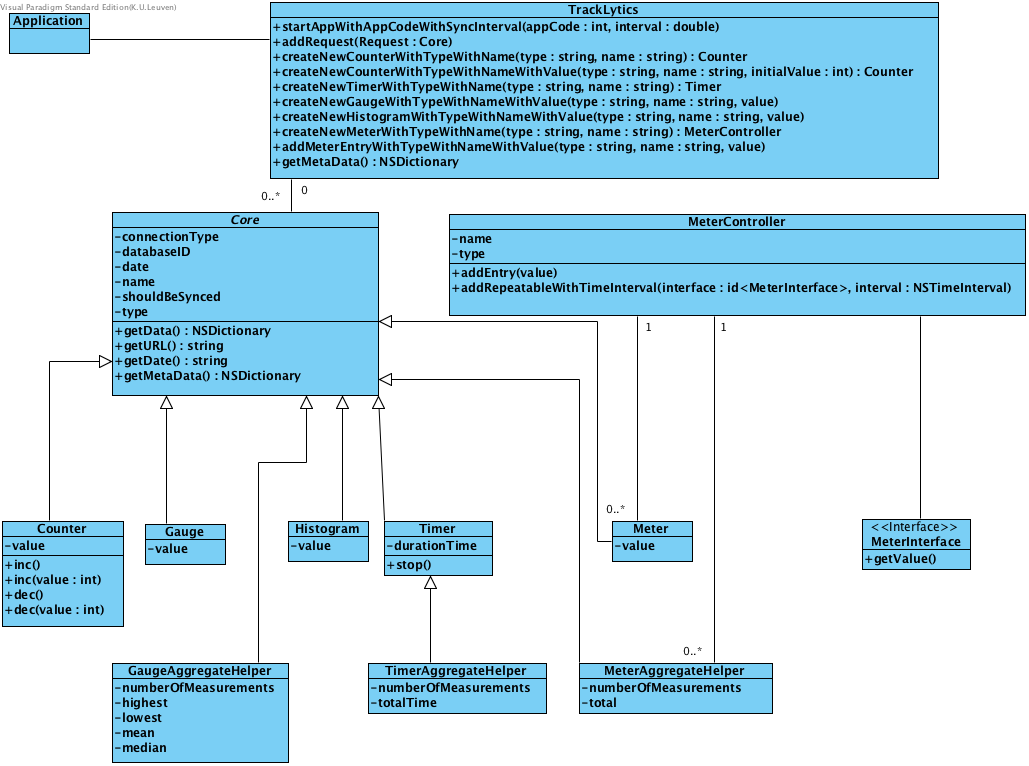
\includegraphics[scale=0.4]{Afbeeldingen/Implementatie/ClassDiagram}
  \caption{Klassediagram Tracklytics library.}
  \label{fig:fig}
\end{figure}

Het klassediagram duidt de klasses aan waaruit de Tracklytics libray bestaat. De verantwoordelijkheden van de verschillende klasses worden uitgelegd in de volgende secties.

\subsection{TrackLytics}
De Tracklytics klasse is de klasse die de synchronisatie met de server verzorgt. De klasse is ook verantwoordelijk voor het creëren en opslaan van de meetobjecten. De klasse heeft enkel statische methodes, dit zorgt ervoor dat er niet telkens opnieuw een instantie van deze klasse aangemaakt moet worden. Dit bespaart enerzijds code, door niet telkens opnieuw een statement te moeten schrijven die de klasse aanmaakt en anderzijds bespaart dit RAM geheugen, omdat de verschillende Tracklytics objecten in het RAM geheugen op het toestel gaan zitten.

\subsection{Core}
Om de gemeenschappelijke elementen te combineren is ervoor gekozen om die gemeenschappelijke elementen in een abstracte superklasse te steken. De gemeenschappelijke methodes worden ook in de Core klasse gestoken, zodat de subklasses indien nodig dit kunnen overriden. 

\subsection{Counter}
De counter klasse stelt een telobject voor. Je kan bij een counter een getal optellen en aftrekken. De inc() functie verhoogt de waarde van de counter met 1 terwijl inc(x) de waarde van de counter verhoogt met x. Dit is opgesplitst omdat inc() vaker gebruikt gaat worden en zo moet er niet telkens inc(1) uitgevoerd worden. Hetzelfde geldt voor dec dat de waarde van de counter gaat verlagen. 

\subsection{Gauge}
De gauge klasse stelt een object met een waarde voor. Dit object wordt aangemaakt en opgeslagen met die waarde en gesynchroniseerd naar de server. Er zijn geen methodes beschikbaar speciaal voor dit object, omdat deze waarde niet aangepast zal worden.

\subsection{Histogram}
De gauge klasse en het histogram zijn maar op 1 punt verschillend en dat is in de back-end. De waarde van het histogram wordt ergens anders opgeslagen dan de waarde van de gauge. In de Tracklytics library hebben ze dezelfde functionaliteit, enkel de URL naar waar de data verstuurd wordt verschilt. Dit zorgt ervoor dat in de back end de data op een andere plaats opgeslagen wordt en het dashboard zo deze data kan onderscheiden.

\subsection{Timer}
De timer klasse kan gebruikt worden om de lengte (in tijd) van een gebeurtenis te meten. Bij het aanmaken van de timer wordt de huidige timestamp bijgehouden. De stop() methode neemt de huidige timestamp en vergelijkt die met degene die werd bijgehouden. Zo weten we de lengte van de gebeurtenis. Indien de programmeur de methode stop() nooit aanroept wordt de timer niet gesynchroniseerd naar de server zodat er geen foute data tussen de data in de database staat. 

\subsection{Meter}
Een meter is bedoeld om een reeks van waarden te kunnen meten. Om dit voor de developer makkelijk te maken zijn er  3 componenten uitgedacht: de Meter, de MeterController en de MeterInterface. De meter component is een uitzondering als er gekeken wordt naar het flow diagram uit de vorige sectie \ref{fig:flow2}. In plaats van dat een Meter object wordt terug gegeven, wordt er een MeterController object terug gegeven. Een MeterController beheert de collectie van de data van Meter waardes. 

\subsubsection{Meter}
Het meter object is het object dat opgeslagen wordt en dat gesynchroniseerd wordt naar de server. Het object houdt de waarde bij en ook het tijdstip van aanmaken. Per meting dat de meter in de applicatie moet er een Meter object aangemaakt worden. Dit is een van de reden dat de MeterController bestaat. 

\subsubsection{MeterController}
De metercontroller zorgt ervoor dat nieuwe meters aangemaakt kunnen worden. De metercontroller bevat de naam en het type van de meter.De keuze om de meters op deze manier aan te maken berust zich op het feit dat zo niet telkens opnieuw het type van de meter moet meegegeven worden, omdat de metercontroller dit al doet en ook om de data periodiek op te kunnen halen. De metercontroller biedt een mogelijkheid aan om via de MeterInterface\ref{Klassediagram:MeterInferface} periodiek een waarde op te halen. Deze functionaliteit zorgt ervoor dat de developer niet telkens na een bepaald interval zelf de metercontroller aan moet roepen, maar dat dit automatisch gebeurt.


\subsubsection{MeterInterface}\label{Klassediagram:MeterInferface}
De meterinterface wordt gebruikt om automatisch een waarde op te halen. De metercontroller roept de enige methode die deze interface aanbiedt (getValue()) aan elke keer een gegeven tijdsinterval voorbij is. De developer moet deze methode implementeren in de klasse waar deze data gecollecteerd moet worden.  


\section{Documentatie}\label{documentatie}
In deze sectie wordt er uit de doeken gedaan hoe je als developer de Tracklytics library in je applicatie kunt inbouwen. 


\subsection{Initialisatie}
De Tracklytics library moet bij het opstarten van de applicatie gestart worden om het synchronisatieproces te starten. De aanbevolen manier is om dit in de \texttt{\justify AppDelegate} klasse te doen in de \texttt{\justify (BOOL)application:(UIApplication *)application didFinishLaunchingWithOptions:(NSDictionary *)launchOptions} methode. Deze methode wordt automatisch uitgevoerd nadat de applicatie opgestart is, in welke applicatie dan ook. In deze methode is het dus belangrijk om volgende code uit te voeren: \texttt{\justify [TrackLytics startTrackerWithAppCode:appCode withSyncInterval:interval];}. Deze code start het synchronisatieproces van de Tracklytics library. De parameter appCode stelt de unieke code voor die Tracklytics gebruikt voor het identificeren van de applicatie. De interval parameter geeft de tijd (in seconden) tussen twee synchronisatiecycli weer. 

\subsection{Counter}
Een counter kan aangemaakt worden met behulp van volgende call naar de Tracklytics library: \texttt{\justify [Tracklytics createNewCounterWithType:type withName:name withValue:value]}, de withValue:value is optioneel indien er een initi\"ele waarde in de counter moet staan. Deze methode geeft een CounterObject terug, wat besproken wordt in volgende sectie. \\

\paragraph{Parameters}
\begin{itemize}
\item type: Het type evenement (bv. Button als er op een button geklikt wordt, vrij te kiezen door de developer). Deze parameter zorgt ervoor dat de data verdeeld wordt over de verschillende grafieken in het dashboard.
\item name: De naam van het evenement (bv. de naam die de button heeft). Deze parameter zorgt ervoor dat de data in de grafieken verder opgedeeld worden per naam.
\item value: De initi\"ele waarde die de counter moet hebben wanneer die gecre\"eerd wordt. Deze waarde is optioneel en is standaard 0 bij creatie.
\end{itemize}

\subsubsection{CounterObject}
Bij de creatie van een Counter wordt er een CounterObject terug gegeven. Dit object kan gebruikt worden om evenementen te tellen. Een counter biedt een methode aan om de counter te verhogen: \texttt{inc} met een optionele waarde. Het object biedt ook een methode aan om de counter te verlangen: \texttt{dec}, ook met een optionele waarde. De Tracklytics library zorgt ervoor dat het CounterObject in sync blijft met de back end. 


\subsection{Gauge}
Aangezien een gauge waarde niet verandert in de tijd, is het niet nodig om hier, zoals bij de counter, een object terug te geven. De waarde moet maar een keer opgeslagen en doorgezonden worden naar de server. Om de waarde op te slaan moet men de volgende methode uitvoeren: \texttt{\justify [Tracklytics createNewGaugeWithType:type withName:name withValue:value]}. 

\paragraph{Parameters}
\begin{itemize}
\item type: Het type evenement (bv. Search Result bij een zoekopdracht). Deze parameter zorgt ervoor dat de data verdeeld wordt over de verschillende grafieken in het dashboard.
\item name: De naam van het evenement (bv. het ingevulde woord/zin in de zoekopdracht). Deze parameter zorgt ervoor dat de data in de grafieken verder opgedeeld worden per naam.
\item value: De waarde die gesynchroniseerd moet worden naar de server (bv. het aantal resultaten van de zoekopdracht).
\end{itemize}

\subsection{Histogram}
Een histogram heeft dezelfde eigenschappen als een gauge in termen van collectie van data in de Tracklytics library. Een histogram waarde verandert niet in de tijd en het is dus niet nodig om een object hiervan terug te geven. De methode die aangeroepen wordt verschilt enkel in de naam van de methode: \texttt{\justify  createNewHistogramWithType:type withName:name withValue:value}. De parameters worden nog eens opgesomd om een goed overzicht te hebben.

\paragraph{Parameters}
\begin{itemize}
\item type: Het type evenement. Deze parameter zorgt ervoor dat de data verdeeld wordt over de verschillende grafieken in het dashboard.
\item name: De naam van het evenement. Deze parameter zorgt ervoor dat de data in de grafieken verder opgedeeld worden per naam.
\item value: De waarde die gesynchroniseerd moet worden naar de server.
\end{itemize}

\subsection{Timer}
Een timer meet de tijd dat een evenement nodig heeft. Om een timer aan te maken moet de volgende call gemaakt worden naar de Tracklytics library: \texttt{\justify [Tracklytics createNewTimerWithType:type withName:name]} 

\paragraph{Parameters}
\begin{itemize}
\item type: Het type evenement. Deze parameter zorgt ervoor dat de data verdeeld wordt over de verschillende grafieken in het dashboard.
\item name: De naam van het evenement. Deze parameter zorgt ervoor dat de data in de grafieken verder opgedeeld worden per naam.
\end{itemize} 

Deze methode geeft een Timer object terug. Vanaf dat deze methode uitgevoerd is begint de timer te lopen. Deze blijft lopen tot de \texttt{\justify stop} methode aangeroepen wordt op het Timer object. De timer heeft dan een exacte waarde hoeveel tijd het evenement in beslag nam. Tracklytics houdt deeze waarde bij en synchroniseert deze naar de server. 


\subsection{Meter}
Een meter is complexer dan alle andere meetobjecten in de Tracklytics library. Dit is omdat ervoor gekozen is om de mogelijkheid aan te bieden om data automatisch op een bepaald interval te collecteren. Zo moet de developer hier niet meer naar omkijken. Om dit te kunnen verwezenlijken is er een controller gemaakt, de MeterController, die de mogelijkheid biedt voor de automatische collectie van data en van de manuele invoer van data. Een MeterController can gecre\"eerd worden door de volgende call naar de Tracklytics library: \texttt{\justify [Tracklytics createNewMeter:type]}. 

\paragraph{Parameters}
\begin{itemize}
\item type: Het type evenement. Deze parameter zorgt ervoor dat de data verdeeld wordt over de verschillende grafieken in het dashboard.
\end{itemize}

\subsubsection{MeterController}
De metercontroller zorgt voor het managen van de meter values. Het is mogelijk om manueel data toe te voegen of automatisch de data te laten controlleren. \\

Om data manueel toe te voegen moet de volgende methode uitgevoerd worden: \texttt{\justify addEntry: (float) value}. De value parameter is de waarde die moet toegevoegd worden aan de meter. \\

Om de date automatisch te laten collecteren moet de methode \texttt{\justify addRepeatable:(id<MeterInterface>) interface withTimeInterval:(NSTimeInterval) interval} uitgevoerd worden. Deze neemt een object dat de MeterInterface implementeerd als parameter en een interval.\\
Het MeterInterface object implementeerd de \texttt{\justify (float) getValue} methode die een float waarde terug geeft die de MeterController kan collecteren door die methode.\\
Het interval geeft aan (in seconden) hoeveel tijd er tussen twee cyclussen zit waarin de waarde opgehaald wordt.




\section{Openstaande uitdagingen}
De implementatie gegeven in deze thesis dekt niet de volledige architectuur uit de vorige sectie. Er blijven dus nog steeds uitdagingen om de library uit te breiden zodat deze dichter aanleunt aan de architectuur. Er worden ook andere uitbreidingen beschreven die niet in de architectuur beschreven worden, maar van even groot belang zijn dan degene die wel in de architectuur beschreven wordt. 

\subsection{AB Testing}
AB testing wordt gebruikt om geleidelijk aan een nieuwe versie van een applicatie of website uit te rollen, zoals beschreven in de architectuur sectie. Het is een uitdaging om dit concept te combineren met de Tracklytics library. Er moet onderzocht worden wat de effici\"entste manier is om AB testing in mobiele applicaties mogelijk te maken.  Een manier om AB testing te gebruiken is om eerst het versienummer voor die gebruiker op te halen in de database. Een niet effici\"ente manier zou dan zijn om per versie een if statement te gebruiken om zo de verschillende karakteristieken van de versie te bepalen. Deze manier is op drie manieren ineffici\"ent, namelijk: de code van de applicatie (en dus ook de grootte op schijf) wordt groter naarmate er meer versies worden gebruikt, door de if statements wordt de applicatie trager en als er een aanpassing moet gebeuren aan een versie of er wordt een versie toegevoegd moet deze nog steeds eerst via de app store als update uitgevoerd worden.


\subsection{Operating systems} %https://www.netmarketshare.com/operating-system-market-share.aspx?qprid=8&qpcustomd=1
De Tracklytics library is ontwikkeld voor iOS, het besturingssysteem van Apple. Er bestaat buiten iOS nog een besturingssysteem dat de moeite waard is om te bekijken, namelijk Android. Op het moment van schrijven is Android de marktleider met een marktaandeel van 59.65\% in de mobiele markt, gevolgd door iOS (32.28\%). De andere mobiele besturingssystemen zijn niet de moeite waard om te bekijken, omdat deze een bijna verwaarloosbare marktaandeel hebben. De toestellen die Android gebruiken zijn verdeeld over vele versies. Op moment van schrijven draait ongeveer een derde van de toestellen op een twee jaar oud besturingssysteem (KitKat 4.4). In contrast, 79\% van de toestellen die op iOS draaien hebben de laatste versie ge\"installeerd (op moment van schrijven). Elke nieuwe versie brengt veranderingen en vernieuwingen met zich mee, wat er voor zorgt dat sommige taken sneller/trager uitgevoerd worden in de ene versie dan in de andere versie. Dit heeft mede de keuze voor iOS gemaakt. \\

De uitdaging die zich hier voordoet is het schrijven van een library voor Android. Dezelfde architectuur kan worden gebruikt voor de library. Er moeten enkele aanpassingen gedaan worden om dit te doen werken. Allereerst moet er een onderscheid gemaakt kunnen worden tussen iOS en Android data. Door telkens het type besturingssysteem door te sturen als metadata is dit mogelijk om het zo in de database te stoppen. Anderzijds is het noodzakelijk in het Android geval om de versie van het besturingssysteem mee door te sturen, zodat er in het dashboard een duidelijke opdeling hiertussen kan gemaakt worden. Dit zorgt er dan weer voor dat het dashboard complexer wordt om te implementeren.

%\cite{website adoption rate}: http://bgr.com/2016/03/15/as-ios-9-adoption-reaches-79-most-android-users-are-still-running-a-painfully-old-os/ 
%ios adaption rate -> https://developer.apple.com/support/app-store/


\subsection{Aggregatie}
In de architectuur beschreven in deze thesis wordt de aggregatie van de data uitgevoerd in de back end wanneer het dashboard de gegevens opvraagt. Het voordeel hieraan is dat de data opgehaald kan worden en enkel verwerkt wordt wanneer deze nodig is. Een nadeel hieraan is dat dit zeer veel CPU kan kosten en zo het dashboard enorm traag maakt. Dit nadeel is gelinkt aan de hoeveelheid gebruikers van de applicatie en het aantal meetpunten in de applicatie. Groeit een van beide of beiden, dan treedt er een extra vertraging op in het aggregeren van de gegevens. Dit probleem kan opgelost worden door op voorhand te aggregeren, dit kan op twee manieren: \textbf{op het toestel zelf} en \textbf{op periodieke intervallen}. Deze sectie berust zich op het feit dat I/O operaties veel trager zijn dan verwerkingsoperaties.\\

De eerste oplossing is om de aggregatie uit te voeren op het toestel zelf. De Tracklytics library kan aangepast worden om in plaats van de data van de meetpunten zelf door te sturen, eerst deze te verwerken op het toestel zelf en die verwerkte data door te sturen naar de server. De back end zal ook moeten aangepast worden om deze data op te slaan zodat deze herbruikt kan worden. Het voordeel hieraan is dat als het dashboard de data opvraagt van de back end, de back end dit sneller zal kunnen doen, omdat er minder data uit de database opgehaald en verwerkt moet worden. Zo is het dashboard bruikbaarder bij grotere schaal. Een nadeel hieraan is dat dit extra verwerkingskracht op het toestel van de gebruiker kost en dus een grotere impact gaat hebben op de vertraging van de applicatie. \\

Een tweede oplossing is om periodiek (bv. \'e\'en keer peer dag) per applicatie de nieuwe data te gaan aggregeren en samenvoegen met de al geaggregeerde data van de voorbije tijdstippen. Deze functionaliteit moet op de servers ge\"implementeerd worden. Het voordeel hieraan is dat indien het dashboard de data opvraagt, enkel de nieuwe data nog moet samengevoegd worden met de al geaggregeerde data. Dit zorgt voor een enorme performance groei van het dashboard. Het nadeel hieraan is dat ofwel er een overzicht moet bijgehouden worden welke data al geaggregeerd is en welke niet, ofwel de verwerkte data telkens uit de database verwijderd moet worden om delen van de dataset niet opnieuw te verwerken. Dit vraagt dus een extra inspanning om te implementeren. \\

Een derde oplossing is om de twee te combineren. Op het toestel wordt een deel van de aggregatie al gedaan en deze geaggregeerde data wordt dan verwerkt op de servers zoals in het vorige deel. Dit geeft een extra prestatiewinst, de verwerking van de geaggregeerde data op de servers gaat sneller, omdat deze al geaggregeerd is. Er is dus minder CPU-tijd nodig om de opdracht af te werken. Indien het dashboard de data opvraagt aan de back end gaat dit ook veel sneller. De combinatie van de nieuwe data en geaggregeerde data gaat veel sneller, omdat er minder data aanwezig is. \\

Een laatste oplossing is om de data te aggregeren wanneer het echt nodig is en deze dan op te slaan. Als de developer of eigenaar van de applicatie het dashboard voor de eerste keer opent, dan wordt deze data geaggregeerd en opgeslagen zoals bij de tweede oplossing. Als de developer of eigenaar het dashboard de volgende keer opent moet enkel de nieuwe data geaggregeerd worden en gecombineerd met de al geaggregeerde data. Deze combinatie wordt dan opnieuw opgeslagen. Dit proces wordt herhaald telkens dat het dashboard van die applicatie geopend wordt. Het voordeel hieraan is dat dit sneller is dan telkens opnieuw alle data te aggregeren. Het nadeel hieraan is dat er moet bijgehouden worden welke data verwerkt is en welke niet. 


\subsection{Alarmen}
%alarmen als bepaalde waarde over iets gaat of als gemiddelde timer hoger wordt dan ...
Om het concept en nut van alarmen uit te leggen is het handig om met een voorbeeld te beginnen. 

Een eigenaar heeft een applicatie ontwikkeld die communiceert met de back end. De eigenaar heeft ervoor gekozen om servers te huren in plaats van zijn eigen servers te bouwen en onderhouden. De eigenaar wil dat er zo weinig mogelijk servers gehuurd moeten worden en dat de gebruiker van de applicatie geen zichtbare vertraging heeft (er toch genoeg servers zijn om de requests te behandelen). Zo kunnen de kosten geminimaliseerd worden en dus de winst gemaximaliseerd. Developers moeten dus servers toevoegen als de servers de requests niet meer aan kunnen en een server verwijderen indien die server overbodig wordt om het werk gedaan te krijgen. 

Om dit mogelijk te maken moet er een trigger of alarm komen die de developers waarschuwt indien de huidige servers het werk niet meer snel genoeg kunnen doen. Dit alarm kan ge\"implementeerd worden in de servers of in de Tracklytics library. \\

Er bestaan al meerdere oplossingen die deze functionaliteit aanbieden op het vlak van servers. Hier wordt niet verder op ingekeken omdat dit niet in de context van deze thesis past. \\

In de Tracklytics library kan er een alarm functionaliteit aangeboden worden. Een developer moet dan in het dashboard aangeven welke parameter welke waarde maximum mag krijgen. Het is ook handig dat de developer een maximum aantal schendingen van deze parameter kan aangeven en dat hij enkele types van metadata kan uitsluiten. (bv. de tijd dat het kost om data van de back end op te halen mag maximum bij 5 verschillende gebruikers boven de 10 seconden liggen op WiFi en 4G). De developer moet ook de tijdspanne aanduiden waarin deze parameters niet overschreden mogen worden. Indien deze drempel overschreden wordt, moet er een waarschuwing gestuurd worden naar de developer. Hierdoor moeten de drie componenten samenwerken (Dashboard, Back end en mobiele library). Het dashboard moet de gegeven paramaters doorgeven aan de back end zodat deze opgeslagen kunnen worden in de database. De mobiele library moet, via de back end, de parameters ophalen. Indien er dan een match is wanneer er nieuwe gegevens worden doorgegeven via de applicatie, dan moet de library nagaan of deze de drempel niet overschrijden. Indien de drempel wordt overschreden, dan moet dit gemeld worden aan de back end. De Tracklytics library moet dan een call doen naar de back end. De back end slaat deze melding op in de database en gaat na of er een alarm verstuurd moet worden. De back end kijkt dus of er in de gegeven tijdspanne meer schendingen geweest zijn dan dat de developer als maximum aangaf. In plaats van elke keer dat er een schending is na te gaan of er een alarm verstuurd moet worden, kan de back end periodiek nagaan of de parameters overschreden worden. Het voordeel hieraan is dat de back end sneller is, omdat de controle niet telkens moet uitgevoerd worden. Het nadeel is dat het alarm bijna een volledige periode later uitgezonden wordt indien de schending van de parameters aan het begin van de periode plaatsvindt. \\

De alarm functionaliteit kan ervoor zorgen dat er zo weinig mogelijk servers gebruikt worden en het geen impact heeft op de kwaliteit van de applicatie en niet zichtbaar is voor de gebruikers. Zo kunnen de kosten geminimaliseerd worden en de winst gemaximaliseerd. 